\documentclass[tikz]{standalone}
\usepackage{amsmath,amssymb}
\usepackage{xcolor}
\usetikzlibrary{positioning,calc}

% Bra-ket macro (to avoid additional dependencies)
\newcommand{\ket}[1]{\lvert #1\rangle}

\begin{document}
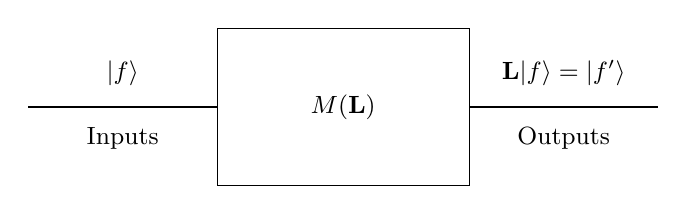
\begin{tikzpicture}[x=1cm,y=1cm, font=\small]
  % -- Size parameters --
  \def\blockW{3.2cm} % Block width
  \def\blockH{2.0cm} % Block height
  \def\xL{-4.0}      % Left x coordinate
  \def\xR{4.0}       % Right x coordinate
  \def\halfW{1.6}    % Half-block width
  \def\halfH{1.0}    % Half-block height

  % -- Block --
  \draw[line width=.4pt] (-\halfW,-\halfH) rectangle (\halfW,\halfH);
  \node at (0,0) {$M(\mathbf{L})$};

  % -- Left and right lines with labels --
  % Left segment: (-4,0) to (-1.6,0)
  \draw[line width=.4pt] (\xL,0) -- (-\halfW,0)
    node[midway, above=4pt] {$\ket{f}$}
    node[midway, below=4pt] {Inputs};

  % Right segment: (1.6,0) to (4,0)
  \draw[line width=.4pt] (\halfW,0) -- (\xR,0)
    node[midway, above=4pt] {$\mathbf{L}\ket{f}=\ket{f'}$}
    node[midway, below=4pt] {Outputs};
\end{tikzpicture}
\end{document}